
% !TEX encoding = UTF-8 Unicode 
% !TEX root = FieldGuide.tex

\Sec{Normal Distribution}
\label{sec:Normal}
\phantomsection\addcontentsline{toc}{subsection}{~~~~~~~~~~~~Normal} 
The  {\bf Normal} (Gauss, Gaussian, bell curve, Laplace-Gauss, de Moivre, error, Laplace's second law of error, law of error)~\cite{Moivre1733,Johnson1994} distribution is a ubiquitous two parameter, continuous, univariate unimodal probability distribution with infinite support, and an iconic bell shaped curve. 
%
\begin{align}
\label{Normal}
\opr{Normal}(x\given \mu,\sigma) 
&=
\frac{1}{\sqrt{2 \pi \sigma^2}}  \exp\left\{ - \frac{( x-\mu)^2}{2\sigma^2} \right\} \checked
\\
& \text{for } x,\ \mu,\  \sigma \text{ in }  \mathbb{R}						\checked 
\notag
\end{align}
The location parameter $\mu$ is the mean, and the scale parameter $\sigma$ is the standard deviation. Note that the normal distribution is often parameterized with the variance $\sigma^2$ rather than the standard deviation. Herein, we choose to consistently parameterize distributions with a scale parameter.  

The normal distribution most often arises as a consequence of the famous central limit theorem, which states (in its simplest form) that the mean of independent and identically distribution random variables, with finite mean and variance, limit to the normal distribution as the sample size becomes large. 
\index{central limit theorem}
The normal distribution is also the maximum entropy distribution for fixed mean and variance.




\SSec{Special cases}
\phantomsection\addcontentsline{toc}{subsection}{~~~~~~~~~~~~Error function}
\phantomsection\addcontentsline{toc}{subsection}{~~~~~~~~~~~~Standard normal}
With $\mu=0$ and $\sigma = 1/ \sqrt{2} h$ we obtain the {\bf error function} distribution, and
with $\mu=0$ and $\sigma=1$ we obtain the {\bf standard normal} ($\Phi$, $z$, unit normal)  distribution. 


 \SSec{Interrelations}
 In the limit that $\sigma\rightarrow\infty$ we obtain an unbounded uniform (flat) distribution, and in the limit $\sigma\rightarrow0$ we obtain a degenerate (delta) distribution. 
 
The normal distribution is a limiting form of many distributions, including the gamma-exponential \eqref{GammaExp}, Amoroso \eqref{Amoroso} and Pearson IV \eqref{PearsonIV} families and their superfamilies. 



Many distributions are transforms of normal distributions.
\begin{align*}
\exp\bigl(\opr{Normal}(\mu,\sigma) \bigr) &\sim \opr{LogNormal}(0, e^\mu, \sigma) & \eqref{LogNormal}  \checked
\\
\big| \opr{Normal}(0,\sigma) \big|  & \sim  \opr{HalfNormal}( \sigma) & \eqref{HalfNormal} \checked
\\
\oprr{StdNormal}{Normal}()^{2} & \sim \opr{ChiSqr}(1)  & \eqref{ChiSqr}  \checked
\\
\sum_{i=1,k}\oprr{StdNormal}{Normal}_i()^{2} & \sim \opr{ChiSqr}(k)  & \eqref{ChiSqr} \checked
\\
\opr{Normal}(0,\sigma)^{-2} & \sim \Levy( 0, \tfrac{1}{\sigma^2})   & \eqref{Levy}  \checked
\\
\big|\opr{Normal}(0,\sigma)\big|^{\tfrac{2}{\beta}} & \sim \opr{Stacy}( (2\sigma^2)^{\tfrac{1}{\beta}}, \tfrac{1}{2}, \beta )  & \eqref{Stacy}  
\\
\frac{\oprr{StdNormal}{Normal}_1()}{\oprr{StdNormal}{Normal}_2()}  & \sim  \opr{StdCauchy}() &\eqref{StdCauchy} \checked
\end{align*}



\begin{figure}[t]
\begin{center}
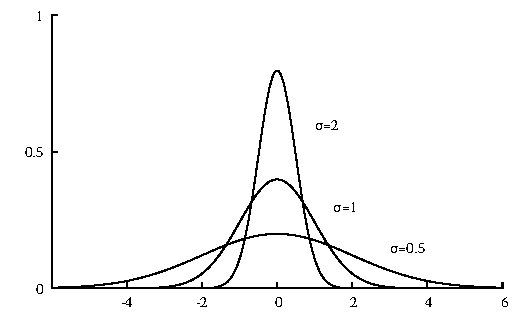
\includegraphics[width=\textwidth]{pdfNormal}
\end{center}
\caption[Normal distributions]{Normal distributions, $\opr{Normal}(x\given 0,\sigma)$}
\end{figure}


The normal distribution is stable \eqref{Stable}. That is a sum of independent normal random variables is also normally distributed.
\[
 \opr{Normal}_1(\mu_1,\sigma_1) +  \opr{Normal}_2(\mu_2,\sigma_2) \sim  \opr{Normal}_3(\mu_1+\mu_2,\sigma_1+\sigma_2)
\checked
\]
\index{stable distributions}

The Box-Muller transform~\cite{Box1958} generates pairs of independent normal variates from pairs of uniform random variates.
\begin{align*}
\oprr{StdNormal}{Normal}_1() & \sim \opr{ChiSqr}(1)\ \cos\bigl( 2\pi\ \opr{StdUniform}_2() \bigr) \checked
\\
\oprr{StdNormal}{Normal}_2() & \sim \opr{ChiSqr}(1)\ \sin\bigl( 2\pi\ \opr{StdUniform}_2() \bigr) \checked
\\
\text{where }& \opr{ChiSqr}(1) \sim\sqrt{ - 2 \ln \opr{StdUniform}_1()}  \checked
\end{align*}
Nowadays more efficient random normal generation methods are generally employed~\secref{sec:random}.




% !TEX encoding = UTF-8 Unicode 
% !TEX root = FieldGuide.tex

\begin{table*}[t!]
\caption[Normal distribution -- Properties]{Properties of the normal distribution}

\begin{align*}
\text{\hyperref[PropertiesSec]{Properties}}  \quad& \\
\text{notation} \quad & \op{Normal}(x\given \mu,\sigma)	\checked
\\
\text{PDF}\quad &   \frac{1}{\sqrt{2 \pi \sigma^2}}  \exp\left\{ - \frac{( x-\mu)^2}{2\sigma^2} \right\} \checked
\\
\text{CDF} \quad  &   \frac{1}{2}\left[  1 + \text{erf}\left(\frac{x-\mu}{\sqrt{2 \sigma^2}} \right) \right]	\checked
\\
\text{parameters}\quad &   \mu,\ \sigma \text{ in } \mathbb{R}						\checked
\\
\text{support} \quad &   x \in [-\infty, + \infty]									\checked
\\
\text{median} \quad  &  \mu												\checked
\\
\text{mode} \quad  & \mu													\checked
\\
\text{mean} \quad  &  \mu													\checked
\\
\text{variance} \quad  & \sigma^2											\checked
\\
\text{skew} \quad  &  0													\checked
\\
\text{kurtosis} \quad  &  0													\checked
\\	
\text{entropy} \quad  & \tfrac{1}{2} \ln(2\pi e \sigma^2)							\checked
\\
\text{MGF} \quad  &  \exp\left({\mu t + \tfrac{1}{2} \sigma^2 t^2 }\right)				\checked
\\
\text{CF} \quad  &  \exp\left({i \mu t - \tfrac{1}{2} \sigma^2 t^2}\right)					\checked
\end{align*}

\end{table*}



